\subsection{Shape Initialization}\label{sec:initialization}

%\cxj{re-write this section. Describe clearly about the parameters, the objective, and methods. }
%In this section we explain the reason why using a specific angle to each fold edge, and constructing our initialized model. 

A general process for humans to fold a carton starts from folding each edge by a rough angle and then connecting close vertexes to obtain a box-like shape. 
Naturally, we first fold the 2D layout by assign an angle to each pair of adjacent faces to get a rough shape, instead of directly computing the vertex coordinates.
%The basic idea is to interpret the folded state of a box as a series of rotation angles along each edge, and by setting specific value of angles which is $\pi/2$, we can have a rough model to assist the later optimization.
%	
Observed from existing data in the Internet, most of the traditional cartons are cuboid for holding files or delivering daily supplies. 
Although there is a recent trend to design more complicated layouts to attract consumers, the shape of these unusual cartons is similar to boxes as their functions are still packaging commodity. 
%
Therefore, we choose $\pi/2$ as the initial value of the rotation angle to each folding edge. 
%
First, a face graph of a layout is constructed, as shown in Figure~\ref{fig:midresult} (a).
Each face is a node, and there is an edge between two faces if there are connected by a folding edge.
%
The faces in the 2D layout are recursively folded in a breadth-first manner.
Starting from the face with the maximal area, our system folds all its adjacent faces by rotate them around their connecting edge by $\frac{\pi}{}$, and then continues to others. 
Figure~\ref{fig:midresult} illustrates the folding process of a cuboid carton. 

\begin{figure}[ht]
	\centering
	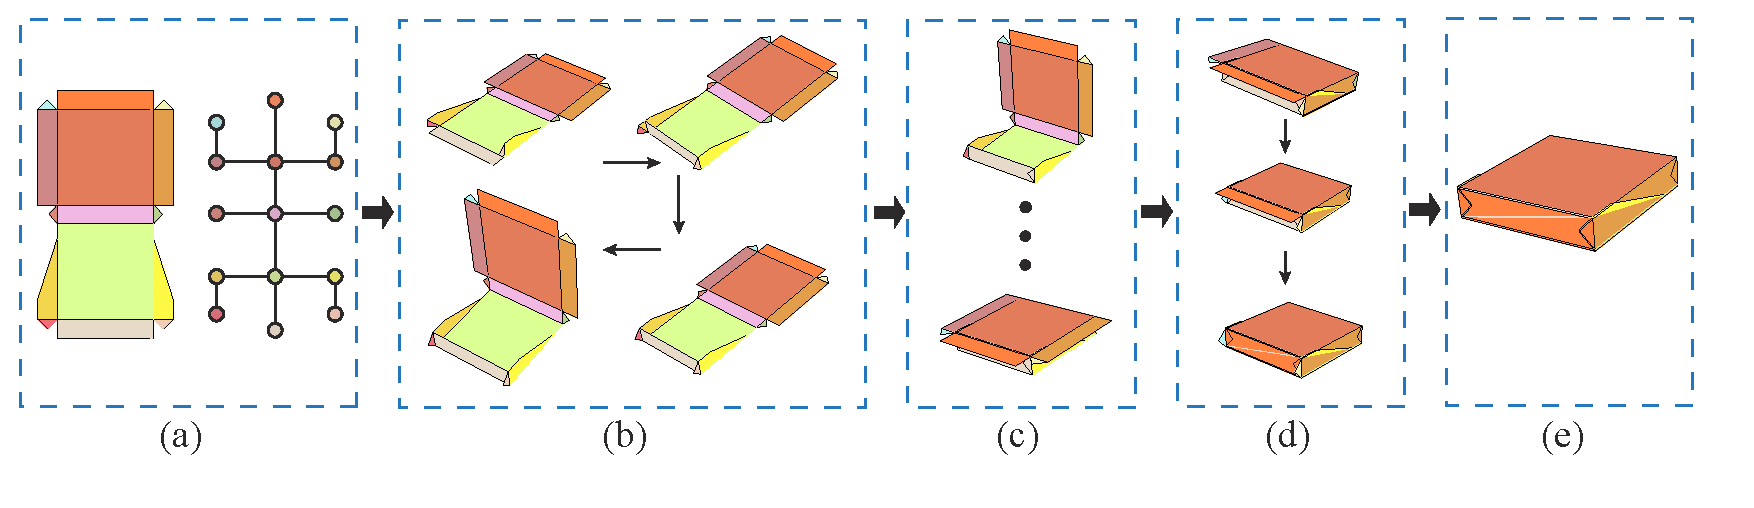
\includegraphics[width=0.9\textwidth]{images/midresult}
	\caption{A rough 3D shape is obtained by folding each face by $\frac{\pi}{2}$ in the 2D layout (a) in a breadth-first manner, starting from the face with the maximum area. (b), (c), (d) and (e) are the different folding stages in the initialization step.}
	\label{fig:midresult}
\end{figure}


Figure~\ref{fig:initial} shows a group of results generated by simply folding faces by $\frac{\pi}{2}$.
Traditional cartons in cuboid shapes could reach an ideal state, as Figure~\ref{fig:initial} shows.
However, many complicated designs still need refinement, such as the four examples in Figure~\ref{fig:initial} (b). 
Take the hexagonal box as an example, the 3D model can be improved by simply snapping the small paste faces to its nearby faces. %
%
As a result, we provide an suggestive interface by automatically detecting potential geometric modifications in the rough carton shape for users to explore.
%interactively allow users to add these constrains into our system and optimize to a desired model, as described in the following section.

\begin{figure}
	\centering
	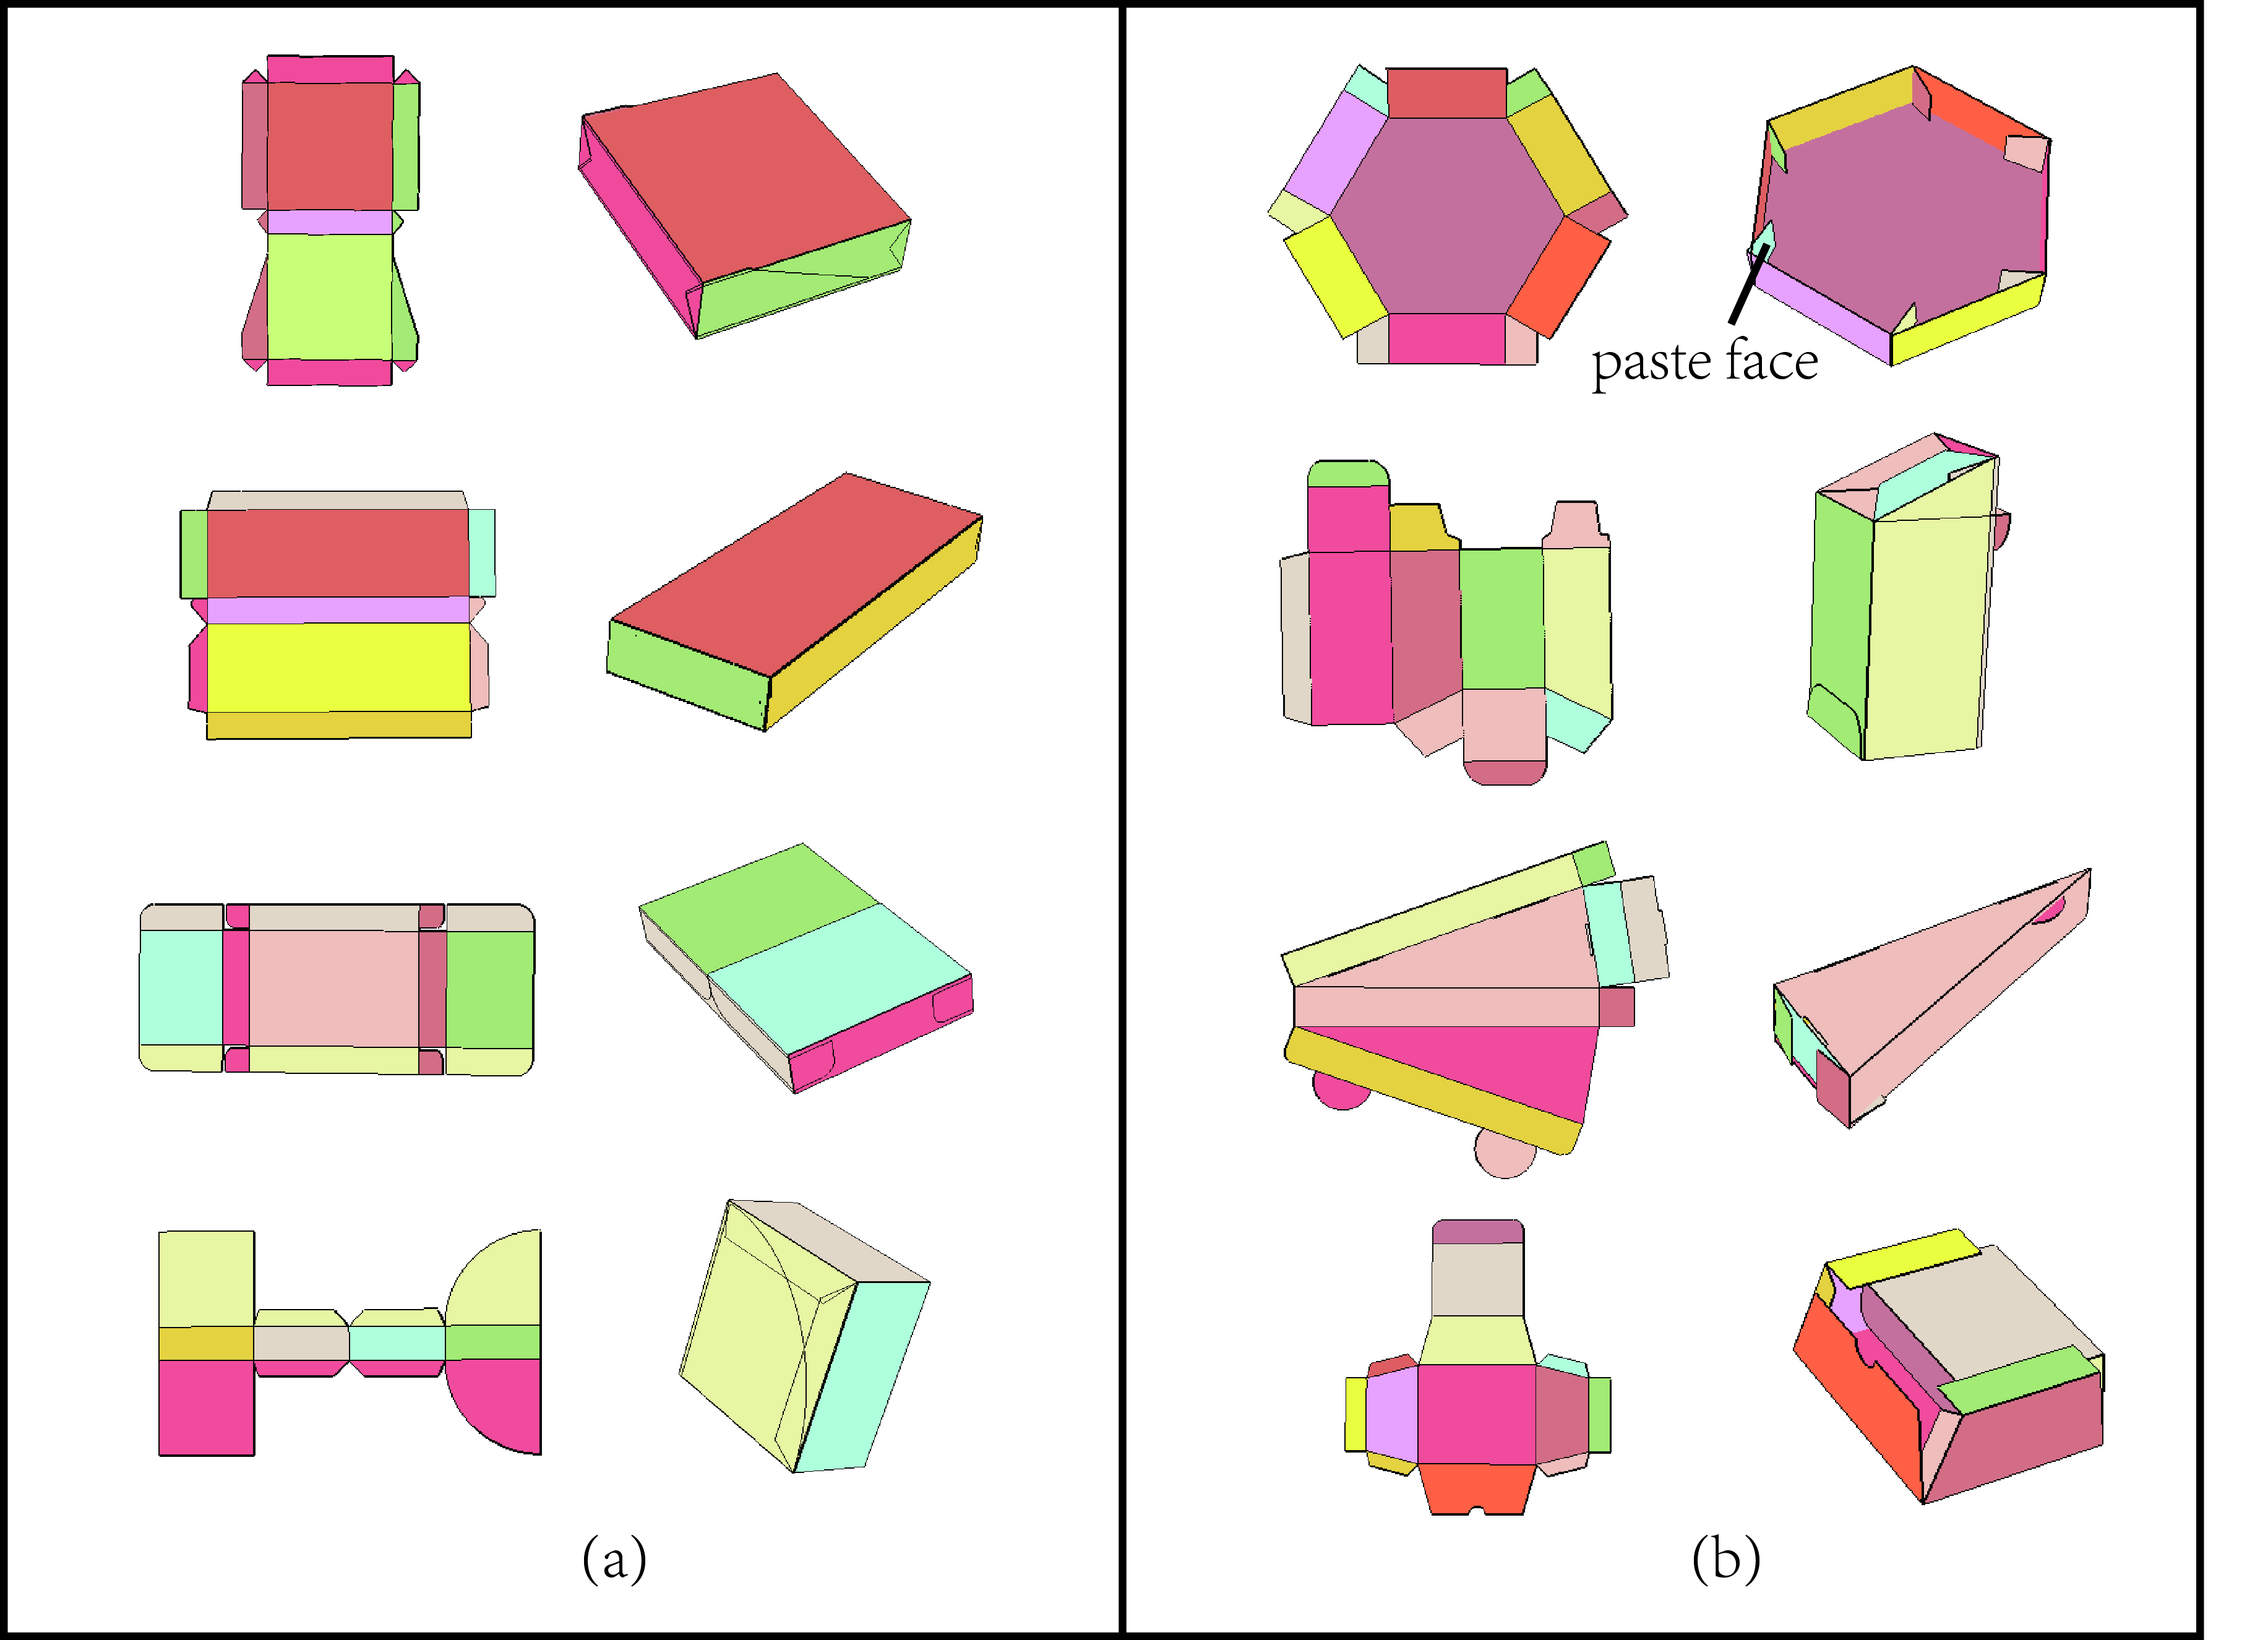
\includegraphics[width=0.9\textwidth]{images/initial.jpg}
	\caption{Eight different initialization results. Four initial cartons shown in the second column of (a) can reach the ideal state, the other four cartons need further refine (b).}
	\label{fig:initial}
\end{figure}

%%%%%%%%%%%%%%%%%%%%%%%%%%%%%%%%%%%%%%%%%%%%%%%%%%%%%%%%%%%%%%%%%%%%%
